\documentclass[12pt,twoside]{article}

\input{macros-sp26}
\newcommand{\thelecturenum}{3}

\title{CS336 Lecture 3}

\begin{document}

\handout{Lecture \thelecturenum: Architectures and Hyperparameters}

\setlength{\parindent}{0pt}

\subsection*{Recapping the Modern Transformer}

Everything you didn't want to know about LM architecture and hyperparameters!

\begin{itemize}
    \item What do most of the large language models (LLMs) have in common?
    \item What are common variations to the architecture / training process?
\end{itemize}

\textbf{Theme:} While the best way to learn is hands-on experience, the next best way is to try to learn from others' experience.  

\subsubsection*{Google's "original" transformer (2017)}

\begin{itemize}
    \item \textbf{Positional embedding:} sines and cosines  
    \begin{align*}
        PE_{(pos, 2i)} &= \sin(pos / 10000^{2i / d_{model}}) \\
        PE_{(pos, 2i + 1} &= \cos(pos / 10000^{2i / d_{model}})
    \end{align*}
    \item \textbf{Feedforward Network (FFN):} ReLU
    \[
        FFN(x) = \max(0, xW_1 + b_1)W_2 + b_2
    \]
    \item \textbf{Norm type:} post-norm, LayerNorm
\end{itemize}

\subsubsection*{CS336's "modern" transformer (2026)}

\begin{itemize}
    \item \textbf{Positional embedding:} Rotary position embedding (RoPE)
    \item \textbf{FFN:} SwiGLU, not ReLU
    \item \textbf{Norm type:} pre-norm, LayerNorm
    \item \textbf{Affine operators:} Linear layers (and layernorm) have no bias (constant) terms
\end{itemize}

\textbf{Questions:} Why did we pick these? What should you pick? \\

Over 19 new \textit{dense} model releases, many of them with minor architecture tweaks ...

\begin{itemize}
    \item Let's look at the data (on dense architectures).
    \item Learn from the many other models (and papers) out there. 
\end{itemize}

\begin{figure}[htbp]
    \centering
    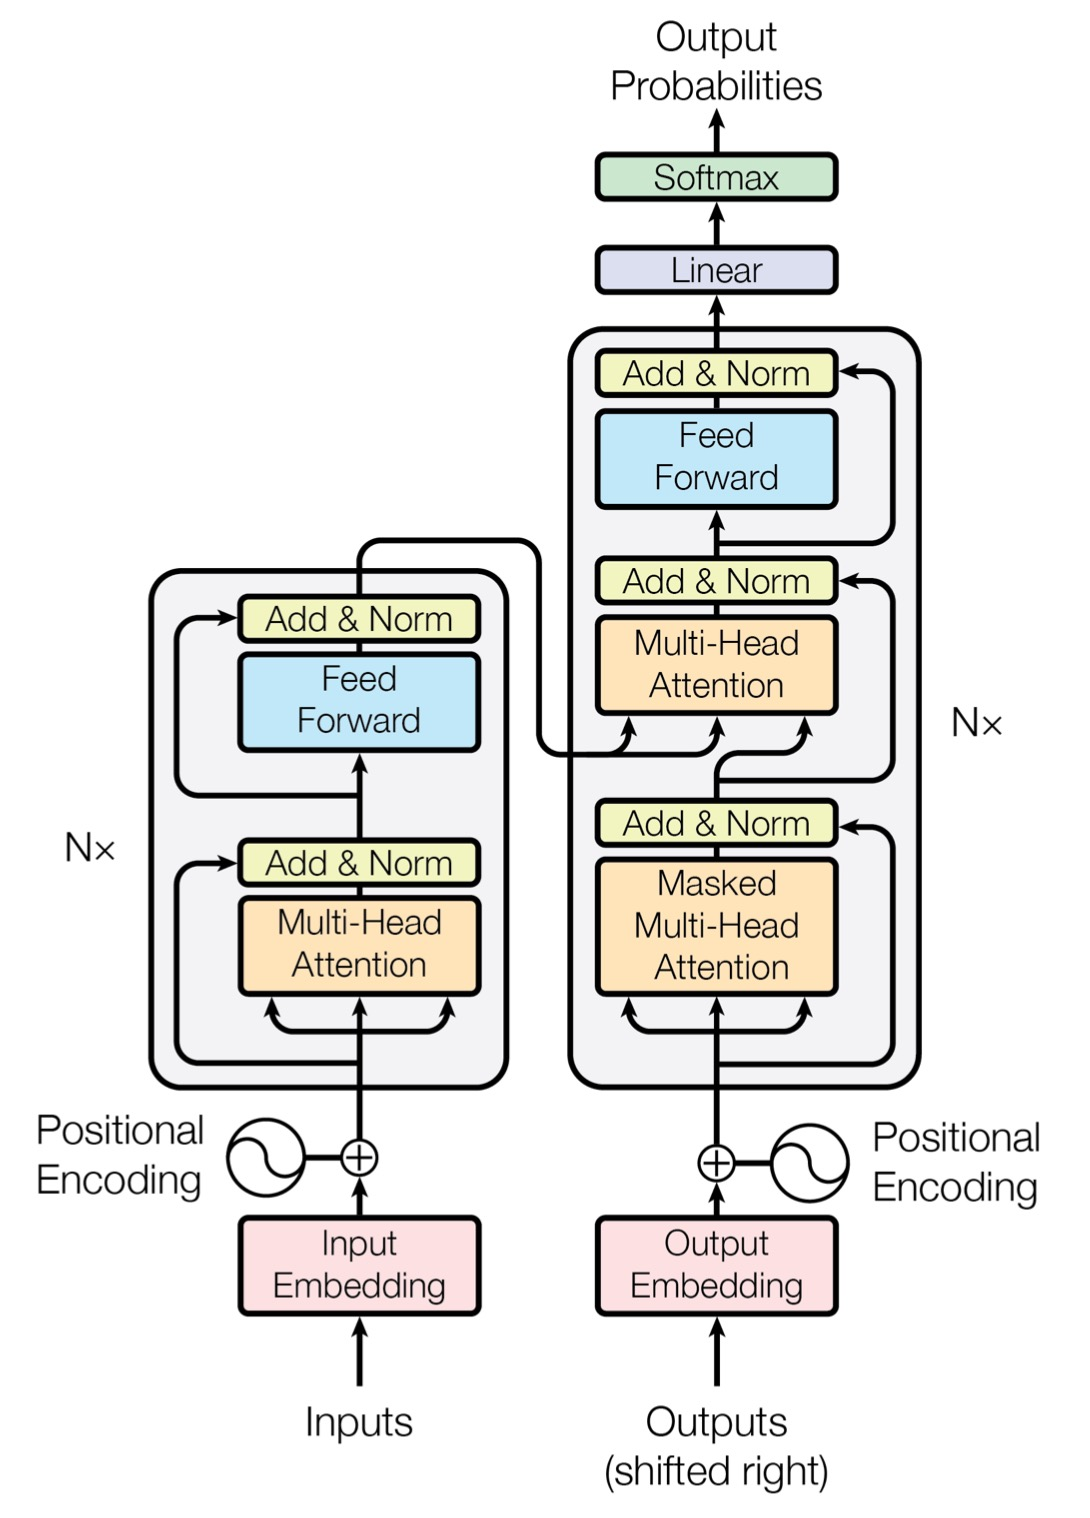
\includegraphics[width=1\linewidth]{transformer.jpeg}
\end{figure}

\begin{figure}[htbp]
    \centering
    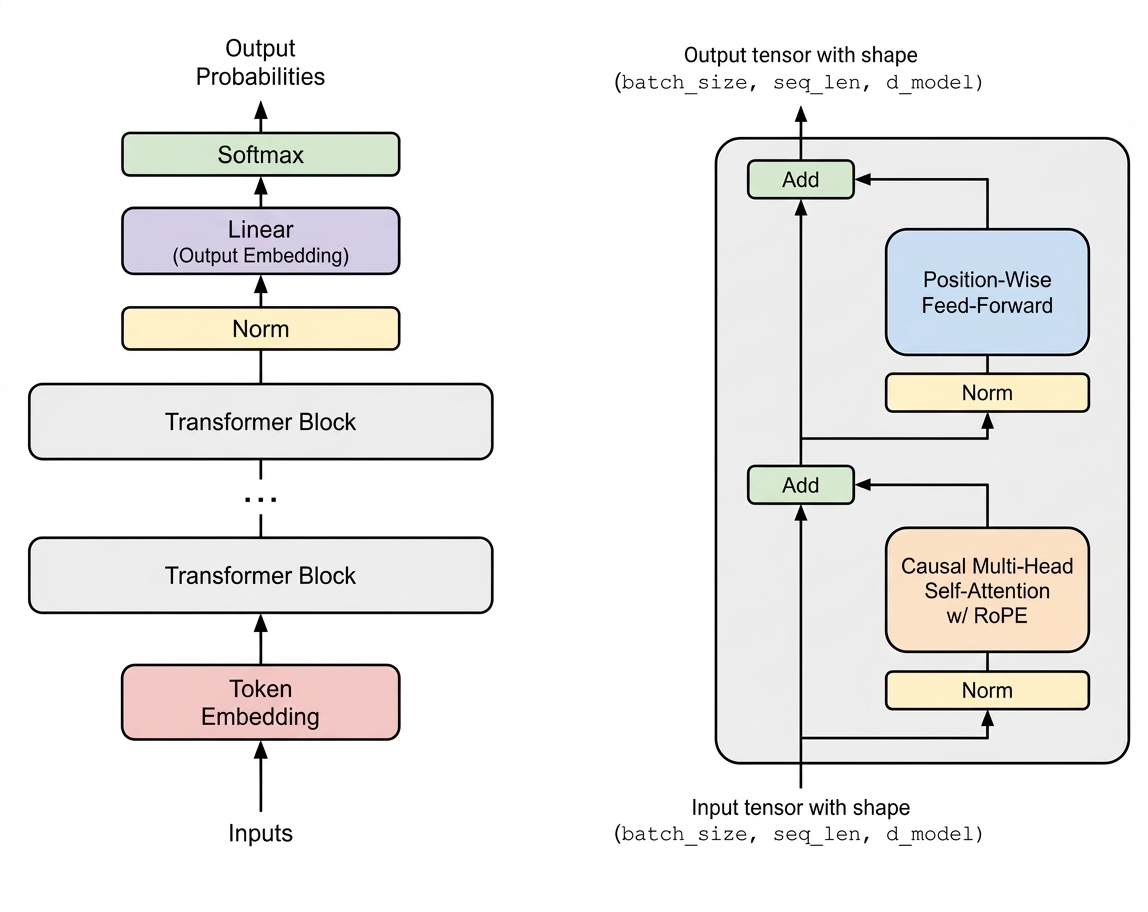
\includegraphics[width=1\linewidth]{modern_transformer.jpg}
\end{figure}

We will talk through many major architecture and hyperparameter variants.

\begin{itemize}
    \item What do all these models have in common?
    \item What parts vary?
    \item What can we learn from this?
\end{itemize}

\textbf{What are we going to cover?}

\begin{itemize}
    \item Activations, feedforward networks
    \item Positional embeddings
    \item Hyperparameters that (do or don't) matter
    \item Stability tricks
    \item Attention variations
\end{itemize}

\textbf{Questions:} What is ff\_dim? Do multi\_head dims always sum to model\_dim? How many vocab elements?

\subsection*{Architecting the Modeling}

Let's think about the core architecture piece:

\begin{itemize}
    \item Dominance of "LLaMA-like" architectures.
    \item Treads over the years (QK-norm, Hybrid attention).
\end{itemize}

\subsubsection*{Pre-vs-Post Norm}

The one thing that \textit{everyone} agrees on (in 2024).

\begin{itemize}
    \item \textbf{Almost all modern LMs use pre-norm (but BERT was post-norm)}.
    \item (One somewhat funny exception - OPT350M. I don't know why this is post-norm).
\end{itemize}

Setup LayerNorm so that it doesn't affect the main residual signal path (on the left). Explanations?

\begin{itemize}
    \item \textbf{Gradient propagation} - nicer attenuation and fewer spikes.
    \item \textbf{Original stated advantage} - removing the warmup.
    \item \textbf{Today} - stability and large learning rates (LRs) for large networks. 
\end{itemize}

\textbf{New things - "double" norm or non-residual post-norms}. 

\begin{itemize}
    \item If putting LayerNorms in residual streams is bad ... Why not post-norm outside the stream?
    \item \textbf{Recent models:} Grok, Gemma 2. Olmo 2 \textit{only} does non-residual post-norm.
\end{itemize}

\subsubsection*{LayerNorm vs RMSNorm}

Original transformer: \textbf{LayerNorm} - normalizes the mean and variance across \(d_{model}\). 

\[
    y = \frac{x - \mathbb{E}[x]}{\sqrt{\sigma^2[x] + \epsilon}} * \gamma + \beta
\]

\textbf{Notable models:} GPT1/2/3, OPT, GPT-J, BLOOM. \\

Many modern LMs: \textbf{RMSNorm} - does not subtract mean or add a bias term.

\[
    y = \frac{x}{\sqrt{\Vert x \Vert^2 + \epsilon}} * \gamma
\]

\textbf{Notable models: } LLaMA-family, PaLM, Chinchilla, T5.

\subsubsection*{Why RMSNorm?}

\textbf{Modern explanation} - it's faster (and just as good).

\begin{itemize}
    \item \textbf{Fewer operations} (no mean calculation).
    \item \textbf{Fewer parameters} (no bias term to store).
\end{itemize}

\textbf{Does this explanation make sense?} MatMuls are the \textit{vast} majority of FLOPs (and memory). \\

\textbf{Important lesson:} FLOPS are not runtime (we will discuss this in far more detail later)! \\

RMSNorm can still matter due to the importance of \textit{data movement} and runtime (plus surprisingly, performance) gains have been seen in papers.

\subsubsection*{More generally: dropping the bias terms}

\begin{remark}
    Most modern transformers don't have bias terms.
\end{remark}

Most implementations (if they're not gated):

\[
    FFN(x) = \sigma(xW_1)W_2.
\]

\textbf{Reason:} memory (similar to RMSNorm) and optimization stability. 

\subsection*{Activating the Neurons}

A whole zoo of activation functions ..

\[
    \text{ReLu, GeLU, Swish, ELU, GLU, GeGLU, ReGLU, SeLU, SwiGLU, LiGLU}
\]

What are these things? What do people use? Does it matter?

\subsubsection*{Common Activations}

\begin{itemize}
    \item \(ReLU(x)= \max(0, x) \implies FFN(x) = \max(0, xW_1)W_2\).
    \item \textbf{Notable models:} Original transformer, T5, Gopher, Chinchilla, OPT. 
    \item \(GeLU(x) = x\Phi(x) \implies FFN(x) = xW_1\Phi(xW_1)W_2\).
    \item \textbf{Notable models:} GPT1/2/3, GPT-J, GPT-Neox, BLOOM.
\end{itemize}

\subsubsection*{Gated Activations (*GLU)}

GLUs modify the "first part" of a FF layer.

\[
    FFN(x) = \max(0, xW_1)W_2
\]

Instead of linear \(+\) ReLU, augment the above with an (entrywise) linear term.

\[
    \max(0,, xW_1) \to \max(0, xW_1) \otimes (xV)
\]

This gives the gated variant (ReGLU) - note that we have an extra parameter (\(V\)).

\[
    FFN_{ReGLU}(x) = (\max(0, xW_1) \otimes xV)W_2
\]

\subsubsection*{Gated Variants of Activations}

\begin{itemize}
    \item \(FFN_{GeGLU}(x, W_1, V, W_2) = (GeLU(xW_1) \otimes xV)W_2\).
    \item \textbf{Notable models:} T5 v1.1, mT5, LaMDA, Phi3, Gemma 2/3/4.
    \item \(FFN_{SwiGLU}(x, W_1, V, W_2) = (Swish(xW_1) \otimes xV)W_2\).
    \item \textbf{Notable models:} LLaMa 1/2/3, PaLM, Mistral, OlMo, \textit{most models post 2023}.
    \item Note: Gated models use smaller dimensions for the \(d_{ff}\) by \(2 / 3\).
\end{itemize}

Do gated linear units work?

\begin{itemize}
    \item Yes, fairly consistently so.
    \item Yes, with other works corroborating Shazeer 2020.
\end{itemize}

\textbf{Many variations (ReLu, GeLU, *GLU) across models.}

\begin{itemize}
    \item*GLU isn't \textit{necessary} for a working model (see GPT3), but it's rare to see others .. some outlier models .. Nemotron 340B (Squared ReLU).
    \item Evidence points towards sonewhat consistent gains from Swi / GeGLU.
\end{itemize}

\subsection*{Serial vs Parallel Layers}

Normal transformer blocks are \textit{serial} - they compute attention, then the MLP.

\begin{question}
    Could we parallelize the transformer block?
\end{question}

A few models (GPTJ, PaLM, GPT-NeoX) do parallel layers. If implemented right, LayerNorm can be shared and matrix multiples can be fused.

\begin{claim}[Recent Models]
    Cohere Command A, Falcon 2 11B, Command R+.
\end{claim}

Most models now use serial layers.

\subsection*{Positioning the Embeddings}

Many variations in positional embeddings ...

\begin{itemize}
    \item \textbf{Sine embeddings:} adds sines and cosines that enable localization
    \[
        Embed(x, i) = v_x + PE_{pos}
    \]
    \item \textbf{Notable models:} original transformer.
    \item \textbf{Absolute embeddings:} add a position vector to the embedding
    \[
        Embed(x, i) = v_x + u_x
    \]
    \item \textbf{Notable models:} GPT1/2/3, OPT.
    \item \textbf{Relative embeddings:} adds a vector to the \textit{attention computation}
    \[
        e_{ij} = \frac{x_iW^Q(x_jW^K + a_{ij}^K)^T}{\sqrt{d_z}}
    \]
    \item \textbf{Notable models:} T5, Gopher, Chinchilla. 
\end{itemize}

\subsubsection*{RoPE: rotary position embeddings}

\textbf{High level thought process:} a \textit{relative} position embedding should be \(f(x, i)\) such that
\[
    \langle f(x, i), f(y, j) \rangle = g(x, y, i - j).
\]

That is, the attention function \textit{only} gets to depend on the relative position (\(i - j\)). 

\begin{question}
    How do existing embeddings not fulfill this goal?
\end{question}

\begin{itemize}
    \item \textbf{Sine:} Has various cross-terms that are not relative
    \[
        \langle Embed(x, i), Embed(y, i) \rangle = \langle v_x, v_y \rangle + \langle PE_i, v_y \rangle ...
    \]
    \item \textbf{Absolute:} obviously not relative
    \item \textbf{Relative embeddings:} \(e_{ij}\) is NOT an inner product
\end{itemize}

\textbf{How can we solve this problem?}

\begin{itemize}
    \item We want our embeddings to be invariant to absolute position.
    \item We know that inner products are invariant to arbitrary rotation.
\end{itemize}

\begin{figure}[hpbt]
    \centering
    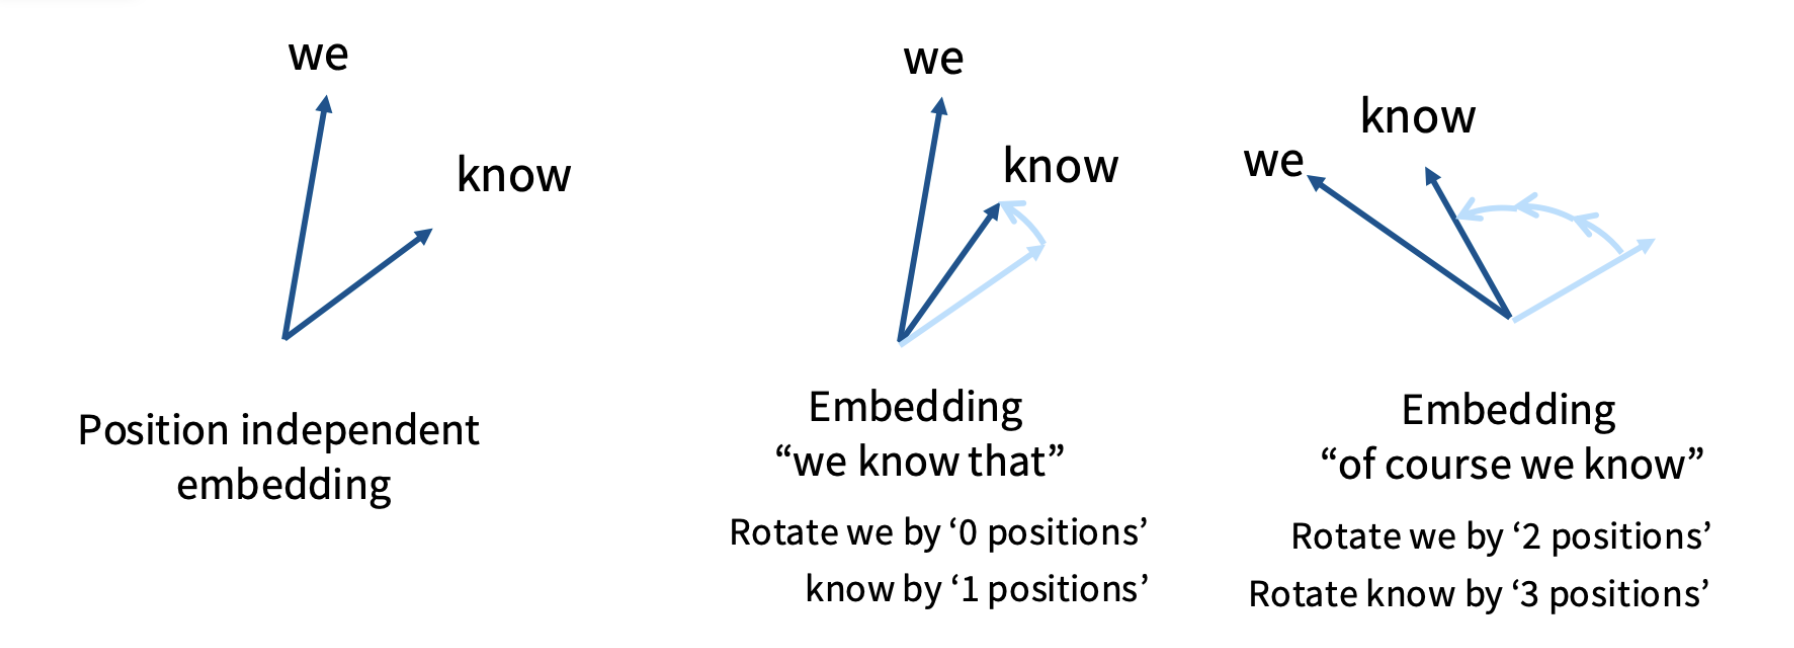
\includegraphics[width=1\linewidth]{RoPE.png}
    \label{fig:placeholder}
\end{figure}

\textbf{There are many rotations, which one do you pick?} Just pair up coordinates and rotate them in 2d (motivation: complex numbers). 

\subsubsection*{The RoPE math}

What is the inner product \(f_{\{q, k\}}\)?
\[
    f_{\{q,k\}}(x_m, m) = R_{\theta, m}^d W_{\{q, k\}} x_m
\]

What is the rotation matrix \(R_{\theta, m}^d\)?
\[
    R_{\theta, m}^{d} = \begin{bmatrix}
        \cos m\theta_1 & -\sin m\theta_1 & 0 & 0 & \cdot \cdot \cdot & 0 & 0 \\
        \sin m\theta_1 & \cos m\theta_1 & 0 & 0 & \cdot \cdot \cdot & 0 & 0 \\
        0 & 0 & \cos m\theta_2 & -\sin m\theta_2 & \cdot \cdot \cdot & 0 & 0 \\
        \vdots & \vdots & \vdots & \vdots & \ddots & \vdots & \vdots \\
        0 & 0 & 0 & 0 & \cdot \cdot \cdot & \cos m\theta_{d / 2} & - \sin m\theta_{d / 2} \\
        0 & 0 & 0 & 0 & \cdot \cdot \cdot & \sin m \theta_{d / 2} & \cos m \theta_{d / 2}
    \end{bmatrix}
\]

Difference with sine embeddings - not additive, no cross terms.

\subsubsection*{Code for RoPE}

\begin{minted}{python}
    query_states = self.q_proj(hidden_states) 
    key_states = self.k_proj(hidden_states)
    value_states = self.v_proj(hidden_states)

    # Flash attention requires the input to have the shape
    # batch_size x seq_length x head_dim x hidden_dim
    # therefore we just need to keep the original shape
    query_states = query_states.view(bsz, q_len, 
        self.num_heads, self.head_dim).transpose(1, 2)
    key_states = key_states.view(bsz, q_len, 
        self.num_key_value_heads, self.head_dim).transpose(1, 2)
    value_states = value_states.view(bsz, q_len, 
        self.num_key_value_heads, self.head_dim).transpose(1, 2)
    
    # Get the RoPE matrix cos/sin
    cos, sin = self.rotary_emb(value_states, position_ids)

    # Multiply query/key inputs
    query_states, key_states = apply_rotary_pos_emb(
        query_states, key_states, cos, sin)
\end{minted}

\textbf{Note:} embedding at \textit{each attention operation} to enforce position invariance.

\subsection*{Engineering the Hyperparameters}

\textbf{Transformer hyperparameter questions you might have had in CS224N ..}

\begin{itemize}
    \item How much bigger should the feedforward size be compared to hidden size?
    \item How many heads and should num\_heads always divide hidden size?
    \item What should my vocab size be?
\end{itemize}

And other model setting questions

\begin{itemize}
    \item Do people even regularize these huge LMs?
    \item How do people scale these models - very deep or very wide?
\end{itemize}

\subsubsection*{Surprising (?) consensus hyperparameter 1}

Feedforward - model dimension ratio.
\[
    FFN(x) = \max(0, xW_1 + b_1)W_2 + b_2
\]

There are two dimensions that are relevant - the feedforward dim (\(d_{ff}\) and model dim (\(d_{model}\)). What should their relationship be?
\[
    d_{ff} = 4 d_{model}
\]

This is \textit{almost always} true. There's just a few exceptions. 

\subsubsection*{Exception \#1 - GLU variants}

Remember that GLU variants scale down by \(2 / 3\). This means most GLU variants have 
\[
    d_{ff} = \frac{8}{3}d_{model}.
\]
Models are roughly in this range, though PaLM, LLaMA2 and Mistral are slightly larger.

\subsubsection*{Exception \#2 - T5}

As we have (and will) see, most LMs are have conservative hyperparameters. One exception is T5 [Raffel et al 2020] which has some \textit{very bold} settings. In particular, for the 11B model, the T5 team set
\begin{align*}
    &d_{ff} = 65,536 \\
    &d_{model} = 1024
\end{align*}

For an astounding 64-times multiplier. 

\begin{center}
    We chose to scale up \(d_{ff}\) specifically because modern accelerators (such as the TPUs we train our models on) are most efficient for large dense matrix multiplications like those in the Transformer's feed-forward network. - Raffel et al 2020
\end{center}

Other, recent exceptions - Gemma 2 (8\(\times\)), SmolLM / Gemma 3 / Gemma 4 (4\(\times\), GLU).

\begin{question}
    Why this range of multiplier?
\end{question}

Empirically, there's a basin between 1-10 where this hyperparameter is near-optimal.

\begin{question}
    What can we learn from the model-dim hyperparameter?
\end{question}

\begin{itemize}
    \item The "default" choices of \(d_{ff} = 4d_{model}\) and \(d_{ff} = 2.66d_{model}\) have worked well for nearly all modern LLMs.
    \item But T5 does show that even radical choices of \(d_{ff} = 64 d_{model}\) can work. This hyperparameter choice isn't written in stone. 
    \item That said, T5 has a follow-up model (T5 v1.1) that is "improved" and uses a much more standrad 2.5 multipler on GeGLU, so the 64-times multipler is likely suboptimal.
\end{itemize}

\subsubsection*{Suprising (?) consensus hyperparameter 2}

Even though we compute \(h\) many attention heads, it's not really more costly.

\begin{itemize}
    \item We compute \(XQ \in \mathbb{R}^{n \times d}\) and then reshape to \(\mathbb{R}^{n \times h \times d / h}\) (likewise for \(XK\) and \(XV\)).
    \item Then we transpose to \(\mathbb{R}^{h \times n \times d / h}\); now the head axis is like a batch axis.
    \item Almost everything else is identical and \textbf{the matrices are the same sizes}.  
\end{itemize}

\begin{claim}
    num-heads \(\times\) head-dimension \(=\) model-dimension. 
\end{claim}

This doesn't \textit{have to} be true: we can have head-dimension \(>\) model-dimension / num-heads. But most models do follow this guideline. 

\begin{remark}
    Most models have around 1 - notable exceptions by some Google models.
\end{remark}

\subsubsection*{Considerations about aspect ratios}

Should my model be deep or wide? \textit{How} deep and how wide?
\[
    \frac{d_{model}}{n_{layer}} \approx 100.
\]

\begin{question}
    Most models are surprisingly consistent on this one too! Sweet spot?
\end{question}

\textbf{Extremely deep models are harder to parallelize and have higher latency}.

\begin{center}
    We note an obvious limitation with our advice. Scaling depth has an obvious limiter, i.e, they are non-parallelization across different machines or devices and every computation has to always wait for the previous layer. This is unlike width, which can be easily parallelizable over thousands or hundreds of thousands of devices. - Tay et al 2021
\end{center}

\begin{question}
    What are typical vocabulary sizes?
\end{question}

\begin{itemize}
    \item Monilingual models: 30-50k words.
    \item Multilingual / production systems: 100-250k words.
\end{itemize}

Monolingual vocabs don't need to be huge, but multilingual ones do.

\subsection*{Dropout and other regularization}

\begin{question}
    Do we need regularization during pretraining?
\end{question}

\textbf{Augments against:}

\begin{itemize}
    \item There is \textit{a lot} of data (trillions of tokens), more than parameters.
    \item SGD only does a single pass on a corpus (hard to memorize). 
\end{itemize}

This is all quite reasonable .. but what do people do in practice?

\begin{itemize}
    \item Many older models used dropout during pretraining.
    \item Newer models (except Qwen) rely only on weight decay. 
\end{itemize}

Most of the times papers just don't discuss dropout. On open models, this closely matches not doing dropout.

\begin{question}
    Why weight decay LLMs?
\end{question}

[Andriushchenko et al 2023] has interesting observations about LLM weight decay.

\begin{itemize}
    \item It's not to control overfitting.
    \item Weight decay interacts with learning rates (cosine schedule).
    \item Its effects are primarily on optimization dynamics. 
\end{itemize}

\subsection*{Stability Tricks}

Recently, lots of attention on \textit{stable training}.

\begin{center}
    Where do the issues arise? Beware of softmaxes! 
\end{center}

\textbf{Softmaxes} - can be ill-behaved due to expomentials / divisions by zero.
\begin{align*}
    \log(P(x)) &= \log\left(\frac{e^{U_r(x)}}{Z(x)}\right) \\
    &= U_r(x) - \log(Z(x)) \\
    Z(x) &= \sum_{r' = 1}^{\vert V \vert} e^{U_r'(x)}
\end{align*}

\subsubsection*{Output softmax stability - "z-loss" trick (Devlin 2014)}

\begin{align*}
    L &= \sum_{i}[\log(P(x_i) - \alpha(\log(Z(x_i)) - 0)^2] \\
    &= \sum_{i}[\log(P(x_i)) - \alpha\log^2(Z(x_i))]
\end{align*}

This is useful for stability! PaLM used this "z-loss" trick.

\begin{center}
    We additionally use an auxiliary loss of \(\Delta z = 10^{-4} \cdot \log^2 Z\) to encourage the softmax normalizer \(\log Z\) to be closer to 0, which we found increases the stability of training.
\end{center}

\textbf{Other examples:} Baichuan 2 (2023), DCLM (2024), OLMo 2/3 (2025).

\subsubsection*{Attention softmax stability - the "QK norm" (Dehgani 2023, Idefcs, Chameleon)}

\begin{itemize}
    \item The query (\(Q\)) and keys (\(K\)) are layer (RMS) normed before going into softmax operation.
    \item \textbf{Other examples:} DCLM, OLMo2, Gemma 2, Qwen3, OLMo 3, Gemma 4.
\end{itemize}

\subsubsection*{Logit soft-capping}

\textbf{Soft-capping} the logits to some maximum value via \(\tanh\). 

\begin{center}
    We cap logits (Bello et al 2016) in each attention layer and the final layer such that the value of the logits stays between \(-\)soft\_cap and \(+\)soft\_cap. More specifically, we cap the logits with the following function:
    \[
        logits \leftarrow softcap * \tanh(logits / softcap).
    \]
\end{center}

Prevents logits from blowing up, but also might have performance issues?

\subsection*{Attending to Heads}

Most models don't touch the attention heads much at all with a few minor exceptions ..

\begin{itemize}
    \item \textbf{GQA / MQA}: Saving inference costs by reducing the number of heads.
    \item \textbf{Sparse or sliding window attention (GPT4 / Mistral)}: restricting the attention pattern to reduce compute cost.
    \item \textbf{Exotic SSM stuff (Jamba, Falcon 3, Qwen 3.5, etc)}: next lecture!
\end{itemize}

\subsubsection*{Reducing attention head cost}

Let's think about the compute involved for attention.
\[
    Atten(X, Q, K, V) = \rho(XQK^TX^T)XV
\]

\textbf{Total arithmetic operations} (\(bnd^2\)) and \textbf{total memory accesses} (\(bnd + bhn^2 + d^2\)). \\

Arithmetic intensity (compute / memory) is high \(O\left((\frac{1}{k} + \frac{1}{bn})^{-1}\right)\) - we can keep our GPUs running.

\begin{question}
    What about the incremental case when we generate text?
\end{question}

\textbf{Key difference:} can't parallelize the generation process - needs to be step by step. 

\begin{remark}
    In this case - we need to incrementally re-compute/update attention via the "KV cache".
\end{remark}

\begin{question}
    What's the incremental arithmetic intensity?  
\end{question}

\textbf{Total arithmetic operations} (\(bnd^2\)) and \textbf{total memory accesses} (\(bn^2d + nd^2\)). \\

Arithmetic intensity is low \(O(\left(\frac{n}{d} + \frac{1}{b}\right)^{-1})\) - we need large batches \(+\) short sequences or big model dimensions. 

\begin{question}
    Is there some way around this? The \(n / d\) term is difficult to reduce.
\end{question}

\subsubsection*{MQA - just have fewer key dimensions}

\textbf{Key idea} - have multiple queries, but just one dimension for keys and values.

\begin{figure}[hpbt]
    \centering
    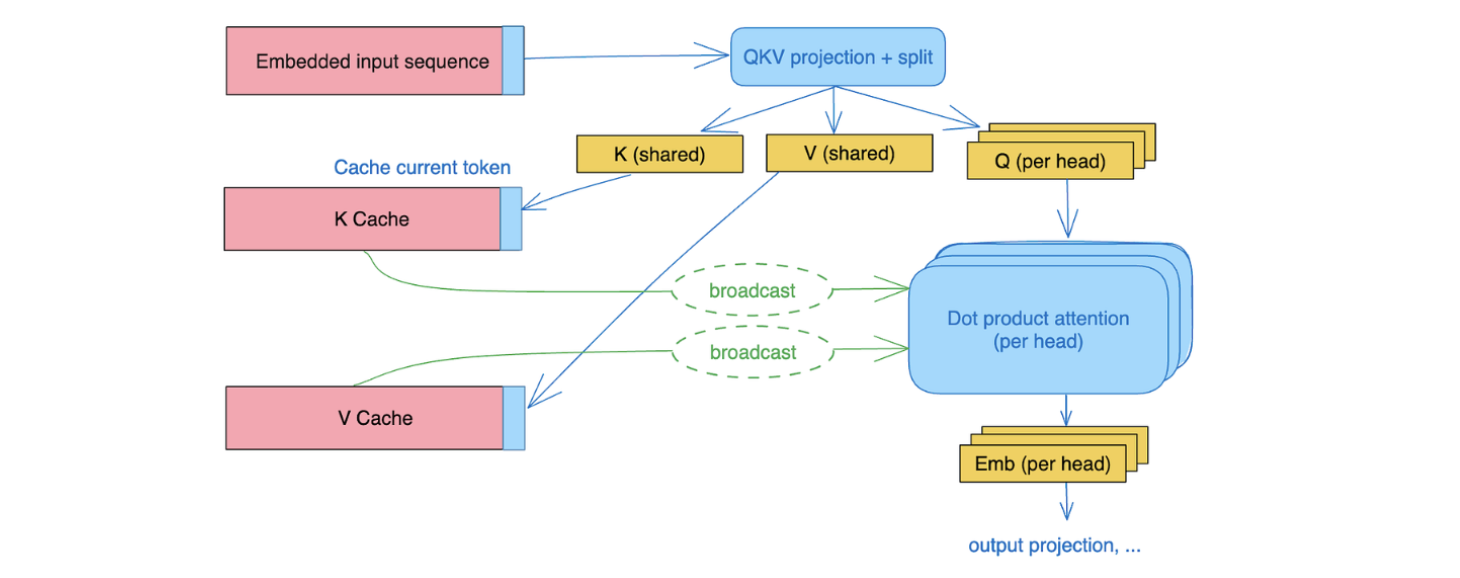
\includegraphics[width=1\linewidth]{MQA.png}
    \label{fig:placeholder}
\end{figure}

\begin{claim}
    We have much fewer items to move in and out of memory (KV cache).
\end{claim}

\textbf{Memory accesses} (\(bnd + bn^2k + nd^2\)) and \textbf{arithmetic intensity} (\(O\left((\frac{1}{d} + \frac{n}{dh} + \frac{1}{b})^{-1}\right)\)).

\subsubsection*{GQA - additional extensions}

Don't do all the way to one dimension of KV - have fewer dimensions.

\begin{figure}[hpbt]
    \centering
    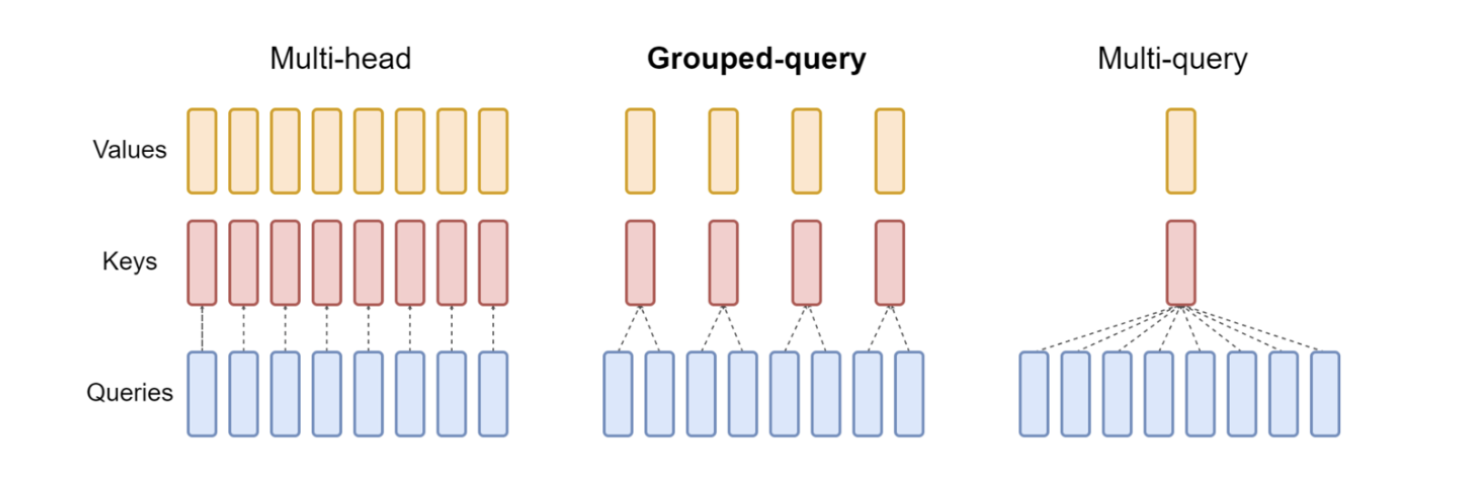
\includegraphics[width=1\linewidth]{GQA.png}
    \label{fig:placeholder}
\end{figure}

\begin{claim}
    Simple knob to control expressiveness (key-query ratio) and inference efficiency. 
\end{claim}

\textbf{More recently} - MLA (multihead latent attention) from DeepSeek v2.

\begin{question}
    Does MQA / GQA hurt? Sometimes ..
\end{question}

\begin{itemize}
    \item Small hit with MQA [Shazeer 2019].
    \item Low hit with GQA [Ainslie 2023].
\end{itemize}

\subsubsection*{Spare / sliding window attention}

\begin{figure}[hpbt]
    \centering
    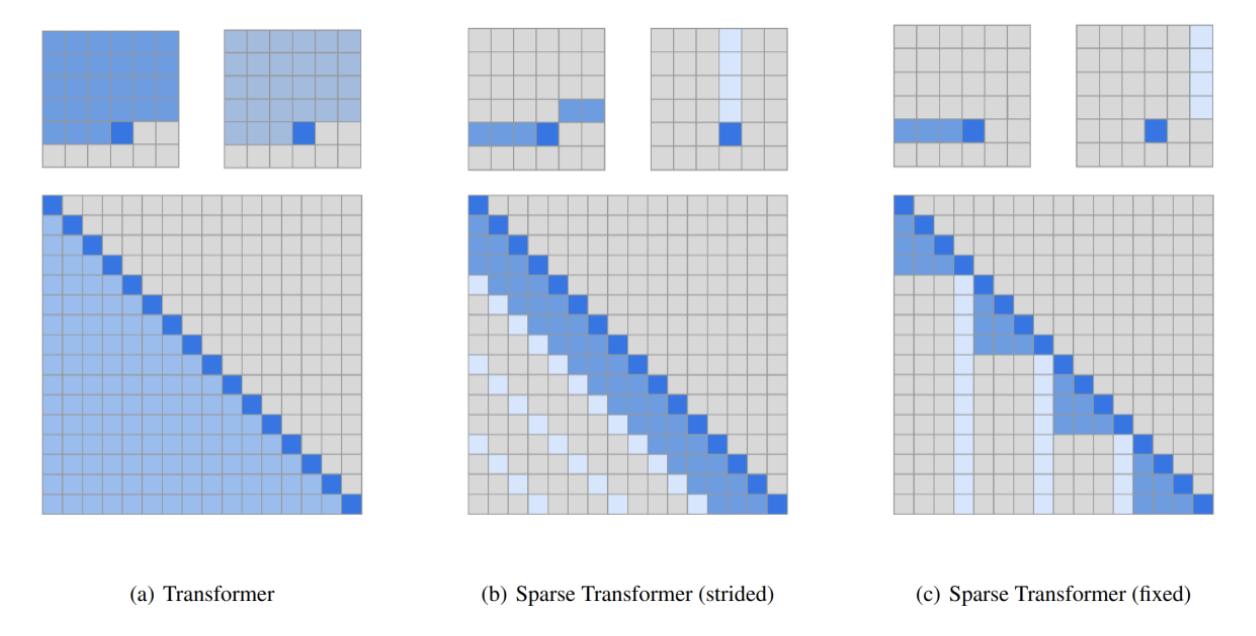
\includegraphics[width=0.75\linewidth]{window.png}
    \label{fig:placeholder}
\end{figure}

\begin{remark}
    Attending to the entire context can be expansive (quadratic). 
\end{remark}

Build sparse / structured attention that trades-off expressiveness verse runtime (GPT3, GPT-OSS, Gemma 4).

\subsubsection*{Current standard trick - interleave "full" and "local" attention}

\begin{itemize}
    \item From Cohere Command A - Every fourth layer is a full attention.
    \item Long-range information via NoPE, short-range information via RoPE \(+\) SWA.
\end{itemize}

\begin{figure}[hpbt]
    \centering
    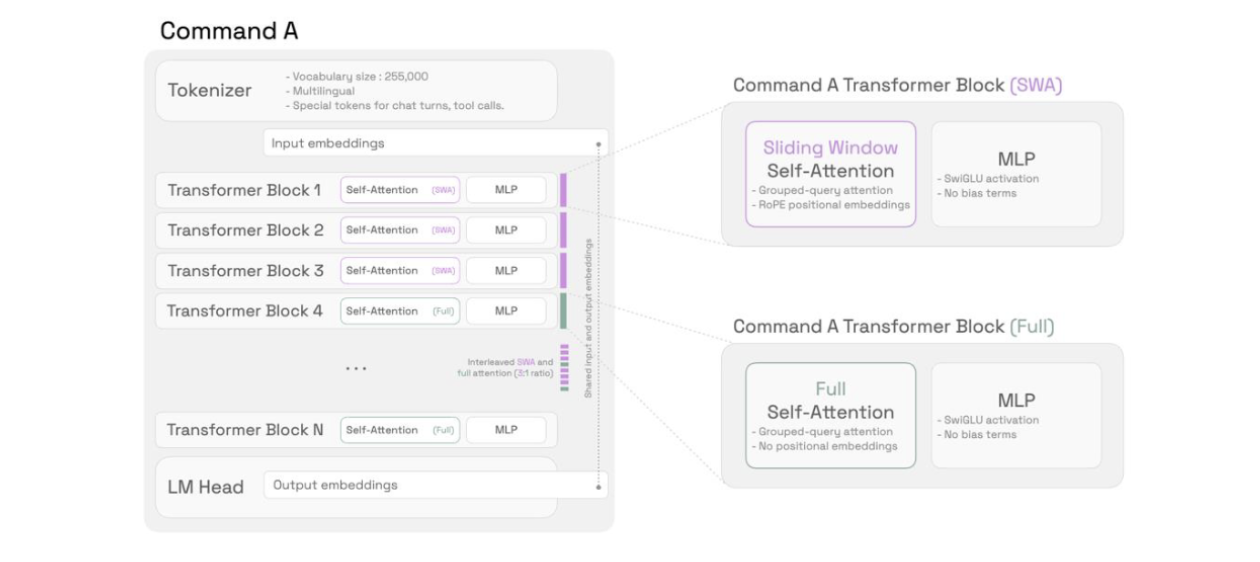
\includegraphics[width=1\linewidth]{command.png}
    \label{fig:placeholder}
\end{figure}

\textbf{Other models} - LLaMA 4, Gemma 3/4, OLMo 3 does SWA \(+\) Full RoPE.

\begin{figure}[hpbt]
    \centering
    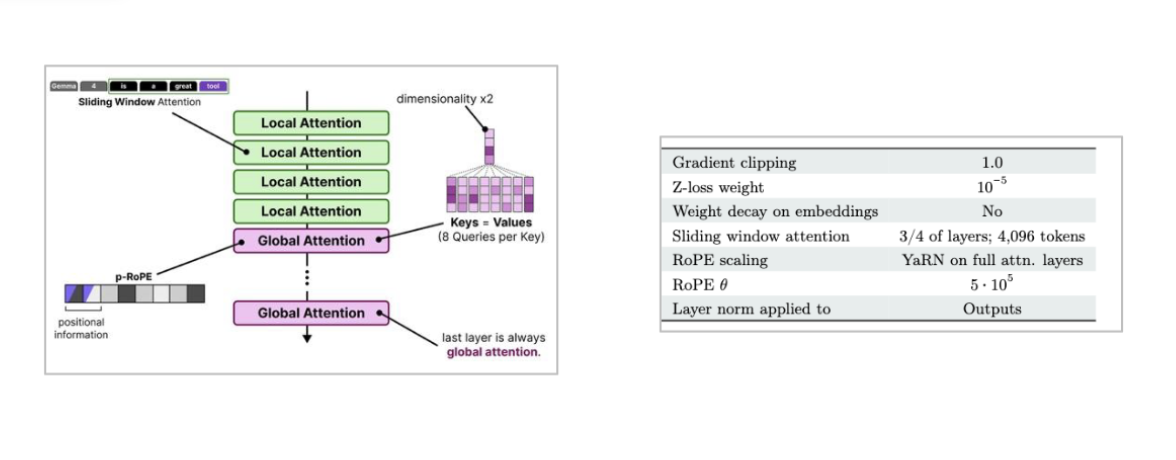
\includegraphics[width=1\linewidth]{others.png}
    \label{fig:placeholder}
\end{figure}

\end{document}
